\documentclass{article}
\usepackage{physics}
\usepackage{graphicx}
\usepackage{caption}
\usepackage{amsmath}
\usepackage{bm}
\usepackage{framed}
\usepackage{authblk}
\usepackage{empheq}
\usepackage{amsfonts}
\usepackage{esint}
\usepackage[makeroom]{cancel}
\usepackage{dsfont}
\usepackage{centernot}
\usepackage{mathtools}
\usepackage{subcaption}
\usepackage{bigints}
\usepackage{amsthm}
\theoremstyle{definition}
\newtheorem{lemma}{Lemma}
\newtheorem{defn}{Definition}[section]
\newtheorem{prop}{Proposition}[section]
\newtheorem{rmk}{Remark}[section]
\newtheorem{thm}{Theorem}[section]
\newtheorem{exmp}{Example}[section]
\newtheorem{prob}{Problem}[section]
\newtheorem{sln}{Solution}[section]
\newtheorem*{prob*}{Problem}
\newtheorem{exer}{Exercise}[section]
\newtheorem*{exer*}{Exercise}
\newtheorem*{sln*}{Solution}
\usepackage{empheq}
\usepackage{tensor}
\usepackage{xcolor}
%\definecolor{colby}{rgb}{0.0, 0.0, 0.5}
\definecolor{MIT}{RGB}{163, 31, 52}
\usepackage[pdftex]{hyperref}
%\hypersetup{colorlinks,urlcolor=colby}
\hypersetup{colorlinks,linkcolor={MIT},citecolor={MIT},urlcolor={MIT}}  
\usepackage[left=1in,right=1in,top=1in,bottom=1in]{geometry}

\usepackage{newpxtext,newpxmath}
\newcommand*\widefbox[1]{\fbox{\hspace{2em}#1\hspace{2em}}}

\newcommand{\p}{\partial}
\newcommand{\R}{\mathbb{R}}
\newcommand{\C}{\mathbb{C}}
\newcommand{\lag}{\mathcal{L}}
\newcommand{\nn}{\nonumber}
\newcommand{\ham}{\mathcal{H}}
\newcommand{\M}{\mathcal{M}}
\newcommand{\I}{\mathcal{I}}
\newcommand{\K}{\mathcal{K}}
\newcommand{\F}{\mathcal{F}}
\newcommand{\w}{\omega}
\newcommand{\lam}{\lambda}
\newcommand{\al}{\alpha}
\newcommand{\be}{\beta}
\newcommand{\x}{\xi}

\newcommand{\G}{\mathcal{G}}

\newcommand{\f}[2]{\frac{#1}{#2}}

\newcommand{\ift}{\infty}

\newcommand{\lp}{\left(}
\newcommand{\rp}{\right)}

\newcommand{\lb}{\left[}
\newcommand{\rb}{\right]}

\newcommand{\lc}{\left\{}
\newcommand{\rc}{\right\}}


\newcommand{\V}{\mathbf{V}}
\newcommand{\U}{\mathcal{U}}
\newcommand{\Id}{\mathcal{I}}
\newcommand{\D}{\mathcal{D}}
\newcommand{\Z}{\mathcal{Z}}

%\setcounter{chapter}{-1}


\usepackage{enumitem}



\usepackage{listings}
\captionsetup[lstlisting]{margin=0cm,format=hang,font=small,format=plain,labelfont={bf,up},textfont={it}}
\renewcommand*{\lstlistingname}{Code \textcolor{violet}{\textsl{Mathematica}}}
\definecolor{gris245}{RGB}{245,245,245}
\definecolor{olive}{RGB}{50,140,50}
\definecolor{brun}{RGB}{175,100,80}

%\hypersetup{colorlinks,urlcolor=colby}
\lstset{
	tabsize=4,
	frame=single,
	language=mathematica,
	basicstyle=\scriptsize\ttfamily,
	keywordstyle=\color{black},
	backgroundcolor=\color{gris245},
	commentstyle=\color{gray},
	showstringspaces=false,
	emph={
		r1,
		r2,
		epsilon,epsilon_,
		Newton,Newton_
	},emphstyle={\color{olive}},
	emph={[2]
		L,
		CouleurCourbe,
		PotentielEffectif,
		IdCourbe,
		Courbe
	},emphstyle={[2]\color{blue}},
	emph={[3]r,r_,n,n_},emphstyle={[3]\color{magenta}}
}






\begin{document}
\begin{framed}
\noindent Name: \textbf{Huan Q. Bui}\\
Course: \textbf{8.421 - AMO I}\\
Problem set: \textbf{\#1}\\
Due: Friday, Feb 11, 2022.
\end{framed}
	
	
\noindent \textbf{1. Driven harmonic oscillator.} It is useful to first have, at our fingertips, the solution for the damped, driven harmonic oscillator:
\begin{equation*}
\ddot x + \gamma \dot x + \omega_0^2 x = \f{F_0}{m}\cos(\omega t)
\end{equation*}
To make the forthcoming algebraic manipulations clearer, let us use complex notations, so that $\cos(\omega t) \to e^{i\omega t}$. Since the problem concerns only the steady-state solution, we shall ignore the transient behavior and consider the following ansatz oscillating at the drive frequency $\omega$:
\begin{align*}
x(t) = A e^{i\omega t } e^{i\phi}
\end{align*}
where $A \in \mathbb{R}$ is the amplitude and $\phi \in \mathbb{R}$ is the phase. Plugging the ansatz into the ODE, we find 
\begin{align*}
x(t) = A e^{i\omega t} e^{i\phi} \implies -A e^{i \omega t + i\phi} \lp \omega^2 -\omega_0^2 - i\gamma \omega \rp = \f{F_0}{m}e^{i\omega t} \implies A = \f{F_0/m}{-\omega^2 + \omega_0^2 + i\gamma \omega} e^{-i\phi}.
\end{align*}
Since $A$ is real, the denominator of $A$ must be a complex number of the form $\abs{A} e^{-i\phi}$ where
\begin{align*}
\abs{A} = \sqrt{{(\omega_0^2 - \omega^2)}^2 + (\gamma \omega)^2}.
\end{align*}
And the phase $\phi$ is\footnote{I should have used $e^{-i\phi}$ so that $\phi$ in this definition would be the phase \textit{lag}...}
\begin{align*}
\boxed{\phi = -\arctan(\f{\gamma\omega}{\omega_0^2 - \omega^2})}
\end{align*}
With these, we may write
\begin{align*}
\boxed{A = \f{F_0/m}{\sqrt{(\omega_0^2 - \omega^2)^2 + (\gamma \omega)^2}}}
\end{align*}
The oscillator is underdamped, so we want the roots of the associated chacteristic polynomial $\lambda^2 + \gamma \lambda + \omega_0^2 = 0$:
\begin{align*}
\lambda\pm = -\f{\gamma}{2} \pm \f{1}{2}\sqrt{\gamma^2 - 4\omega_0^2}
\end{align*}
to be complex (to get oscillations on top of an exponential decay). As a result, we require that 
\begin{align*}
\gamma^2 < 4\omega_0^2 \iff \boxed{\gamma < 2\omega_0}
\end{align*}






\begin{enumerate}[label= \alph*)]
	\item We want to find $\omega$ for which:
	
	\begin{enumerate}[label=\roman*)]
		\item $A$ is maximal. Before proceeding, let us introduce two dimensionless quantities $\rho = \omega/\omega_0$ and $f = \gamma/\omega_0$ and rewrite $A$ as 
		\begin{align*}
		A =  \lp \f{F_0}{m \omega_0^2}\rp \f{1}{\sqrt{(1-\rho^2)^2 + (f\rho)^2}}
		\end{align*}
		Finding $\omega$ so that $A$ is maximal requires finding $\rho$ for which the denominator of $A$ is minimal:
		\begin{align*}
		\f{d}{d\rho}\lb (1-\rho^2)^2 + (f\rho)^2 \rb = 2\rho(-2 + f^2 + 2\rho^2).
		\end{align*}
		Setting the expression above to zero tells us that $\rho$ could be $0$ or $\sqrt{1-f^2/2}$ (we must also verify that $A$ has a global maximum, but I won't go into the details here). Since $f = \gamma/\omega_0 \in (0,2)$ we must consider two cases:
		\begin{itemize}
			\item If ${0 < f \leq \sqrt{2}}$ then the solution $\rho = \sqrt{1-f^2/2}$ is real and we have 
			\begin{align*}
			A(0)= \f{F_0}{m\omega_0^2} <  \f{F_0}{m\omega_0^2} \lp \f{2}{f\sqrt{4-f^2}}\rp  = A\lp \sqrt{1-f^2/2}\rp
			\end{align*}
			because $f\sqrt{4-f^2} \leq 2$ for $f\in (0,2)$. We therefore see that $A$ attains its maximum at $$\omega = \omega_0 \sqrt{1- \gamma^2/2\omega_0^2}.$$
			
			
			
			\item Otherwise, if ${\sqrt{2} < f < 2}$ then the solution $\rho = \sqrt{1-f^2/2}$ is imaginary and $A$ attains its maximum of $F_0/m\omega_0^2$ at $$\omega = 0.$$
		\end{itemize}
	
	
	
	\item The phase \textit{lag} being $\pi/2$ means that $\phi = -\pi/2$, i.e.,
	\begin{align*}
	\arctan\lp \f{\gamma \omega}{\omega_0^2 - \omega^2} \rp = \f{\pi}{2} \implies \omega = \omega_0.
	\end{align*}
	
	
	\item The power from the drive is given by $P = dW/dt$ where $dW$ is the work done by the drive over an infinitesimal $dx$ and is thus given by $dW = Fdx$.  Putting everything together we have $P = F(t)x'(t)$. The power delivered from the drive, averaged over one cycle of period $T = 2\pi / \omega$, is therefore
	\begin{align*}
	\langle P \rangle 
	&= \f{\omega}{2\pi}\int_{0}^{2\pi/\omega} F_0 \cos(\omega t) \f{d}{dt} \Re{x(t)} \,dt \\
	&= \f{F_0 A \omega}{2\pi}  \int_{0}^{2\pi/\omega} \cos(\omega t)  \f{d}{dt} \cos\lp \omega t + \phi \rp \,dt \\
	&= -\f{F_0 A \omega^2}{2\pi}  \int_{0}^{2\pi/\omega} \cos(\omega t) \sin\lp \omega t + \phi \rp \,dt \\
	&= -\f{1}{2}F_0 A \omega \sin \phi.
	\end{align*} 
	Plugging in the expressions for $\phi$ and $\omega$ we find 
	\begin{align*}
	\langle P \rangle = \f{F_0^2 }{2m\gamma}\f{(\gamma\omega)^2}{(\omega_0^2 - \omega^2)^2 + (\gamma \omega)^2}.
	\end{align*}
	We recognize that $P$ has the form of a Lorentzian (or a Cauchy distribution) with FWHM $\gamma$ which attains the maximum $\langle P \rangle_\text{max} = F_0^2/2m\gamma$ at $\omega = \omega_0$.  \textcolor{blue}{One may also use standard calculus techniques to get this result.}
	
	
	$\boxed{\textbf{!}}$ It makes sense that the power delivered by the drive to the oscillator, averaged over one cycle, is the same as the power dissipated by the damping, averaged one cycle, since the system is in equilibrium in steady state. This can be verified by repeating the calculation above explicitly, but for the damping force. The work done by drag force is $-m\gamma x'(t)$, from which we find the dissipated power is $P_\text{dis} = Fv = m\gamma v(t)^2$. From here, we have
	\begin{align*}
	\langle P_\text{dis}\rangle = \f{\omega}{2\pi}m\gamma A^2\int_0^{2\pi/\omega} \lp \f{d}{dt}\cos(\omega t + \phi)\rp^2\,dt = \f{1}{2}m\gamma A^2\omega^2.
	\end{align*}
	Plugging in the expression for $A$ we find that
	\begin{align*}
	\langle P_\text{dis}\rangle = \f{F_0^2}{2m\gamma} \f{(\gamma\omega)^2}{(\omega_0^2 - \omega^2)^2 + (\gamma \omega)^2} = \langle P \rangle \,\,\,\checkmark
	\end{align*}
	\qed
	
	
	
	
	$\boxed{\textbf{?}}$ \textbf{Why does the dissipated power become maximal at that frequency? } Physically, when the drive $F \propto \cos (\omega t)$ is at $\omega = \omega_0$, the position $x(t) \propto \cos(\omega_0 t + \phi)$ of the oscillator has a $-\phi =\pi/2$ phase lag compared to the drive. However, the velocity $x'(t) \propto -\sin(\omega_0 t -\pi/2) = \cos(\omega_0 t)$ is now in phase with the drive. As a result, the drive is always doing positive work, and thus $\langle P \rangle$ is maximal.  
	
	
	\end{enumerate}
	
	\item In the far off-resonance regime, we may assume that $\abs{\omega_0^2 - \omega^2}\gg \gamma \omega$, so that 
	\begin{align*}
	\langle P \rangle_\text{far off res.}  \approx   \f{F_0^2}{2m\gamma} \f{(\gamma \omega)^2}{(\omega_0^2 - \omega^2)^2} \propto \gamma,
	\end{align*}
	so $\langle P \rangle$ varies linearly in $\gamma$ for far off-resonance drive. In the near-resonance regime, we may ignore the term $\omega_0^2 - \omega^2$ in the denominator to find 
	\begin{align*}
	\langle P \rangle_\text{near res.} \approx \f{F_0}{2m\gamma} \propto \gamma^{-1}.
	\end{align*}
	$\boxed{\textbf{?}}$ \textbf{Why does reducing the damping increase the power dissipated on resonance?} The power dissipated goes like $\gamma A^2$. On resonance, the term $\omega_0^2 - \omega^2$ becomes small, and $A^2\sim 1/\gamma^2$, giving us the result we got just above. Therefore we could say that the math tells us that on resonance, reducing the damping increases the power dissipate. Intuitively, however, we could also say that on resonance, the driving force and velocity are in phase. Therefore the power, which goes like $\vec{F} \cdot \vec{v}$, increases as there is less damping  because $\abs{F}$ is fixed and $\abs{v}\sim \abs{A}$ is increased. 	 
	
	
	
	
	\item Now we have resonant driving, so $\omega = \omega_0$. The steady-state average energy stored in the oscillator is the sum of kinetic and potential energy. 
	\begin{align*}
	\langle KE\rangle &= \f{\omega_0}{2\pi} \int_0^{2\pi/\omega_0} \f{1}{2}m x'(t)^2\,dt=   \f{F_0^2 }{4m\gamma^2}\\
	\langle PE \rangle &= \f{\omega_0}{2\pi}\int_0^{2\pi/\omega_0} \f{1}{2}m \omega_0^2 x(t)^2\,dt  = \f{F_0^2}{4m\gamma^2}
	\end{align*}
	where we have used $x(t) = (F_0/m\gamma \omega_0) \sin(\omega_0 t)$. From here, the total energy stored in the oscillator is 
	\begin{align*}
	\langle E \rangle = \langle KE \rangle + \langle PE \rangle = \f{F_0^2}{2m\gamma^2}.
	\end{align*}
	On the other hand, the energy dissipated in one cycle may be calculated by integrating the dissipated power over a cycle $E_\text{lost} = \int P_\text{dis}\,dt$ where $P_\text{dis} = F_\text{damp} v(t)$: 
	\begin{align*}
	E_\text{lost} = \int_0^{2\pi/\omega_0} \gamma m x'(t) x'(t)\,dt = \f{F_0^2 \pi}{m\gamma \omega_0}.
	\end{align*}
	Take the $2\pi$-adjusted ratio of these two results, we find 
	\begin{align*}
	2\pi \f{\langle E \rangle}{E_\text{lost}} = \f{\omega_0}{\gamma},
	\end{align*}
	which is nothing but the quality factor $Q$!
	
\end{enumerate} 



\noindent \textbf{2. Harmonically bound electron - Lorentz model.}


\begin{enumerate}[label=\alph*)]
	\item In view of the result of the previous problem, we can immediately write down the solution $d(t) = ex(t)$ by making the appropriate identifications plus the fact that $\gamma=0$:
	\begin{align*}
	d(t) = ex(t) = \f{e^2 E\cos(\omega t)}{\omega_0^2 - \omega^2}.
	\end{align*}
	
	\item Let us take the resonance case $\omega = \omega_0$. Taking the amplitude of $x(t)$ to be $x_0$, the total power radiated in the full solid angle of $4\pi$ is 
	\begin{align*}
	P = \f{1}{6\pi \epsilon_0 c^3}\abs{\ddot d}^2 = \f{e^2 x_0^2 \omega_0^4 \cos^2(\omega_0 t)}{6 c^3 \pi \epsilon_0}.
	\end{align*}
	The energy lost per orbital cycle is thus
	\begin{align*}
	E_\text{lost} = \int_0^{2\pi/\omega_0} P\,dt = \f{e^2 x_0^2 \omega_0^3}{6c^3 \epsilon_0}.
	\end{align*}
	
	
	\item The total energy is calculated in the same manner as before:
	\begin{align*}
	\langle KE\rangle &= \f{\omega_0}{2\pi} \int_0^{2\pi/\omega_0} \f{1}{2}m x'(t)^2\,dt= \f{1}{4}m \omega_0^2 x_0^2  \\
	\langle PE \rangle &= \f{\omega_0}{2\pi}\int_0^{2\pi/\omega_0} \f{1}{2}m \omega_0^2 x(t)^2\,dt  = \f{1}{4}m \omega_0^2 x_0^2 \\
	E_\text{stored} &= \langle KE \rangle + \langle PE \rangle = \f{1}{2}m \omega_0^2 x_0^2
	\end{align*}
	From here, we get
	\begin{align*}
	Q = 2\pi \f{E_\text{stored}}{E_\text{lost}} = \f{6c^3 m\pi \epsilon_0}{e^2 \omega_0}.
	\end{align*}
	Since $Q = \omega_0 / \Gamma_{\text{rad}}$, we find
	\begin{align*}
	\Gamma_\text{rad} = \f{\omega_0}{Q} = \f{e^2 \omega_0^2}{6c^3 m \pi \epsilon_0}.
	\end{align*} 
	
	\item In terms of the classical radius of the electron
	\begin{align*}
	r_0 = \f{e^2}{4\pi \epsilon_0 mc^2}, 
	\end{align*}
	we have
	\begin{align*}
	Q = \f{3\lambdabar}{2r_0} \quad\quad \text{and}\quad\quad \Gamma_\text{rad} = \f{\omega_0}{Q} = \f{2r_0c}{3\lambdabar^2}
	\end{align*}
	
	\item With $\lambda = 589 $ nm, we have
	\begin{align*}
	Q &\approx 5.0 \times 10^7 \\
	\Gamma_\text{rad} &\approx 2\pi \times 10.2 \text{ MHz}
	\end{align*}
	which is in remarkable agreement with the experimentally measured natural line width for the D2 line of Na which is $2\pi \times 9.795(11)$ MHz. The calculation is within $\sim 5$\% of the measured value.  
\end{enumerate}






\noindent \textbf{3. Quantum harmonic oscillator.} \\


\noindent $\boxed{\textbf{?}}$ \textbf{How are the annihilation and creation operators $ a$ and $ a^\dagger$ relate to $ x$ and $ p$?} Let $a = A  x - i B  p$, where $A,B$ are real scalars, so that $ a^\dagger = A x+ i B  p$. We want the following to hold:
\begin{align*}
\ham = \f{p^2 }{2m} + \f{1}{2}m\omega^2 x^2 = \hbar \omega \lp a^\dagger a + \f{1}{2} \rp
\end{align*}
so we compute
\begin{align*}
\hbar \omega \lp a^\dagger a+ \f{1}{2}\rp = \hbar \omega A^2 x^2 + \hbar \omega B^2 p^2 + \hbar \omega AB + \f{\hbar \omega}{2}
\end{align*}
where we have used $[x,p] = i\hbar $. By setting 
\begin{align*}
A = \sqrt{\f{m\omega}{2\hbar}} \quad\quad B = -\sqrt{\f{1}{2\hbar m\omega}}
\end{align*}
the first equation is satisfied. We therefore conclude that
\begin{align*}
a = \sqrt{\f{m\omega}{2\hbar}} \lp x + \f{i}{m\omega} p \rp \quad\quad a^\dagger = \sqrt{\f{m\omega}{2\hbar}} \lp x - \f{i}{m\omega} p \rp.
\end{align*}
From here, we find 
\begin{align*}
x = \sqrt{\f{\hbar}{2 m\omega}}(a^\dagger + a) \quad\quad p = i\sqrt{\f{\hbar m\omega }{2}}(a^\dagger - a)
\end{align*}

\begin{enumerate}[label=\alph*)]
	\item From the results above, we get
	\begin{align*}
	\bra{n} x \ket{n} = \sqrt{\f{\hbar}{2 m\omega}}\bra{n} a^\dagger + a \ket{n} = 0
	\end{align*}
	\begin{align*}
	\bra{n} p \ket{n} = i\sqrt{\f{\hbar m\omega }{2}}\bra{n} a^\dagger - a \ket{n} = 0
	\end{align*}
	since both $a^\dagger$ and $a$ respectively send $\ket{n}$ to $\ket{n+1}$ and $\ket{n-1}$ which are orthonormal to $\ket{n}$. Next, 
	
	
	\begin{align*}
	\sqrt{\bra{n}p^2 \ket{n}} &= \sqrt{-\f{\hbar m\omega}{2}\bra{n} (a^\dagger - a)^2 \ket{n} }\\
	&= \sqrt{-\f{\hbar m\omega}{2} \bra{n} a^\dagger a^\dagger -a^\dagger a - aa^\dagger + a^2 \ket{n} }\\
	&= \sqrt{\hbar m\omega \lp n+ \f{1}{2} \rp}.
	\end{align*}
	
	\begin{align*}
	\sqrt{\bra{n}x^2 \ket{n}} &= \sqrt{\f{\hbar}{2 m\omega}\bra{n} (a^\dagger + a)^2 \ket{n} }\\
	&= \sqrt{\f{\hbar}{2 m\omega}\bra{n} a^\dagger a^\dagger +a^\dagger a + aa^\dagger + a^2 \ket{n} }\\
	&= \sqrt{\f{\hbar}{m\omega}\lp n+ \f{1}{2} \rp}.
	\end{align*}
	
	
	\item The total energy is 
	\begin{align*}
	\langle  E\rangle  = \f{\langle p^2\rangle }{2m} + \f{1}{2}m\omega^2 \langle x^2\rangle = \f{1}{2m}\hbar m\omega \lp n+ \f{1}{2} \rp + \f{1}{2}m\omega^2 \f{\hbar}{m\omega}\lp n+ \f{1}{2} \rp  = \hbar \omega\lp n+ \f{1}{2}\rp \,\,\, \checkmark
	\end{align*}
	
	Virial theorem: Since $V\propto x^2$, the virial theorem states that $\langle T \rangle  = \langle V \rangle$. From the calculation above, we see that this holds:
	\begin{align*}
	\langle T \rangle =  \f{1}{2m}\hbar m\omega \lp n+ \f{1}{2} \rp  = \f{1}{2}m\omega^2 \f{\hbar}{m\omega}\lp n+ \f{1}{2} \rp = \langle V \rangle \,\,\, \checkmark
	\end{align*}
	
	\item Sketch of $\psi_0(x)$ and $\psi_1(x)$. Here the harmonic potential is proportional to $x^2$. 
	
	
	\begin{figure}[!htb]
		\begin{subfigure}{0.5\textwidth}
			\centering
			\includegraphics[width=\textwidth]{n_0.eps}
		\end{subfigure}
		\begin{subfigure}{0.5\textwidth}
			\centering
			\includegraphics[width=\textwidth]{n_1.eps}
		\end{subfigure}
	\end{figure}
	
	
	
	\item For a Na atom in the state $\ket{0,0,0}$ of a 3D harmonic potential, we have, by spherical symmetry:
	\begin{align*}
	\sqrt{\langle r^2\rangle} = \sqrt{3\langle x^2 \rangle } = \sqrt{3(2\cdot 0+1)\f{\hbar}{2m\omega}} = \sqrt{\f{3\hbar}{2m\omega}}.
	\end{align*}
	With $\omega = 2\pi \times 100 $ Hz and $m_\text{Na} \approx 23 \times 1.66054\times 10^{-27}$ kg, the rms size is
	\begin{align*}
	\sqrt{\langle r^2\rangle} \approx 2.57 \text{ \textmu m}.
	\end{align*}
	
	
	Similarly, we can find the rms velocity using spherical symmetry:
	\begin{align*}
	\sqrt{\langle v^2 \rangle} = \f{1}{m}\sqrt{\langle p^2 \rangle} = \f{1}{m}\sqrt{3\langle p_x^2 \rangle} = \f{1}{m}\sqrt{3(2\cdot 0 + 1) \f{\hbar m \omega}{2}} = \sqrt{\f{3\hbar \omega}{2m}}.
	\end{align*}
	The numerical value for this is
	\begin{align*}
	\sqrt{\langle v^2 \rangle} \approx 1.61 \text{ mm/s}.
	\end{align*}

\end{enumerate}




\end{document}








